\documentclass%[handout]%
{beamer}
%\usetheme{Execushares}
\usetheme{AnnArbor}
\usecolortheme{beaver}
%\setbeamercolor{title}{parent=structure,bg=green!50!black,fg=white}
%\usecolortheme{dolphin}
\setbeamertemplate{navigation symbols}{}%remove navigation symbols

\usepackage{amsmath}
\usepackage{amssymb}
\usepackage{amsthm}
%\usepackage[utf8]{inputenc}
\usepackage[czech]{babel}
\usepackage{tikz-cd}
\usepackage[mathscr]{euscript}
\usepackage[IL2]{fontenc}
\usepackage{mathtools}

\usetikzlibrary{calc,shapes.callouts,shapes.arrows}

%\usepackage{beamerarticle}

%\usepackage{bbm}

\def\rllap#1{\hbox to0pt{\hss#1\hss}}

\newcommand{\bubblethis}[2]{
        \tikz[remember picture,baseline]{\node[anchor=base,inner sep=0,outer sep=0]%
        (#1) {\underline{#1}};\node[overlay,cloud callout,callout relative pointer={(-0.2cm,+0.7cm)},%
        aspect=2.5,fill=yellow!90] at ($(#1.north)+(-0.5cm,1.6cm)$) {#2};}%
    }%
		
\newcommand{\speechthis}[2]{
        \tikz[remember picture,baseline]{\node[anchor=base,inner sep=0,outer sep=0]%
        (pom) {#1};\node[overlay,ellipse callout,fill=blue!50] 
        at ($(pom.north)+(1cm,+0.8cm)$) {#2};}%
    }%
		

\title{Diferenciální a integrální počet}
\author{Alexander Slávik} %  and J. Trlifaj
\subtitle{Úvod, snad motivační}
\institute{Gymnázium Voděradská}
\date{2. 9. 2020}

\begin{document}


\frame{\titlepage}

\section{Úvod}

\begin{frame}
	\frametitle{Historie}
	\pause
	\hbox to\hsize{%
	\hfil
	\vbox{\halign{\hfil####\hfil\cr
	\includegraphics[height=.6\pdfpageheight]{leibniz.jpg}\cr
	Gottfried Wilhelm Leibniz\cr
	1646--1716\cr
	}}%
	\hfil
	\vbox{\halign{\hfil####\hfil\cr
	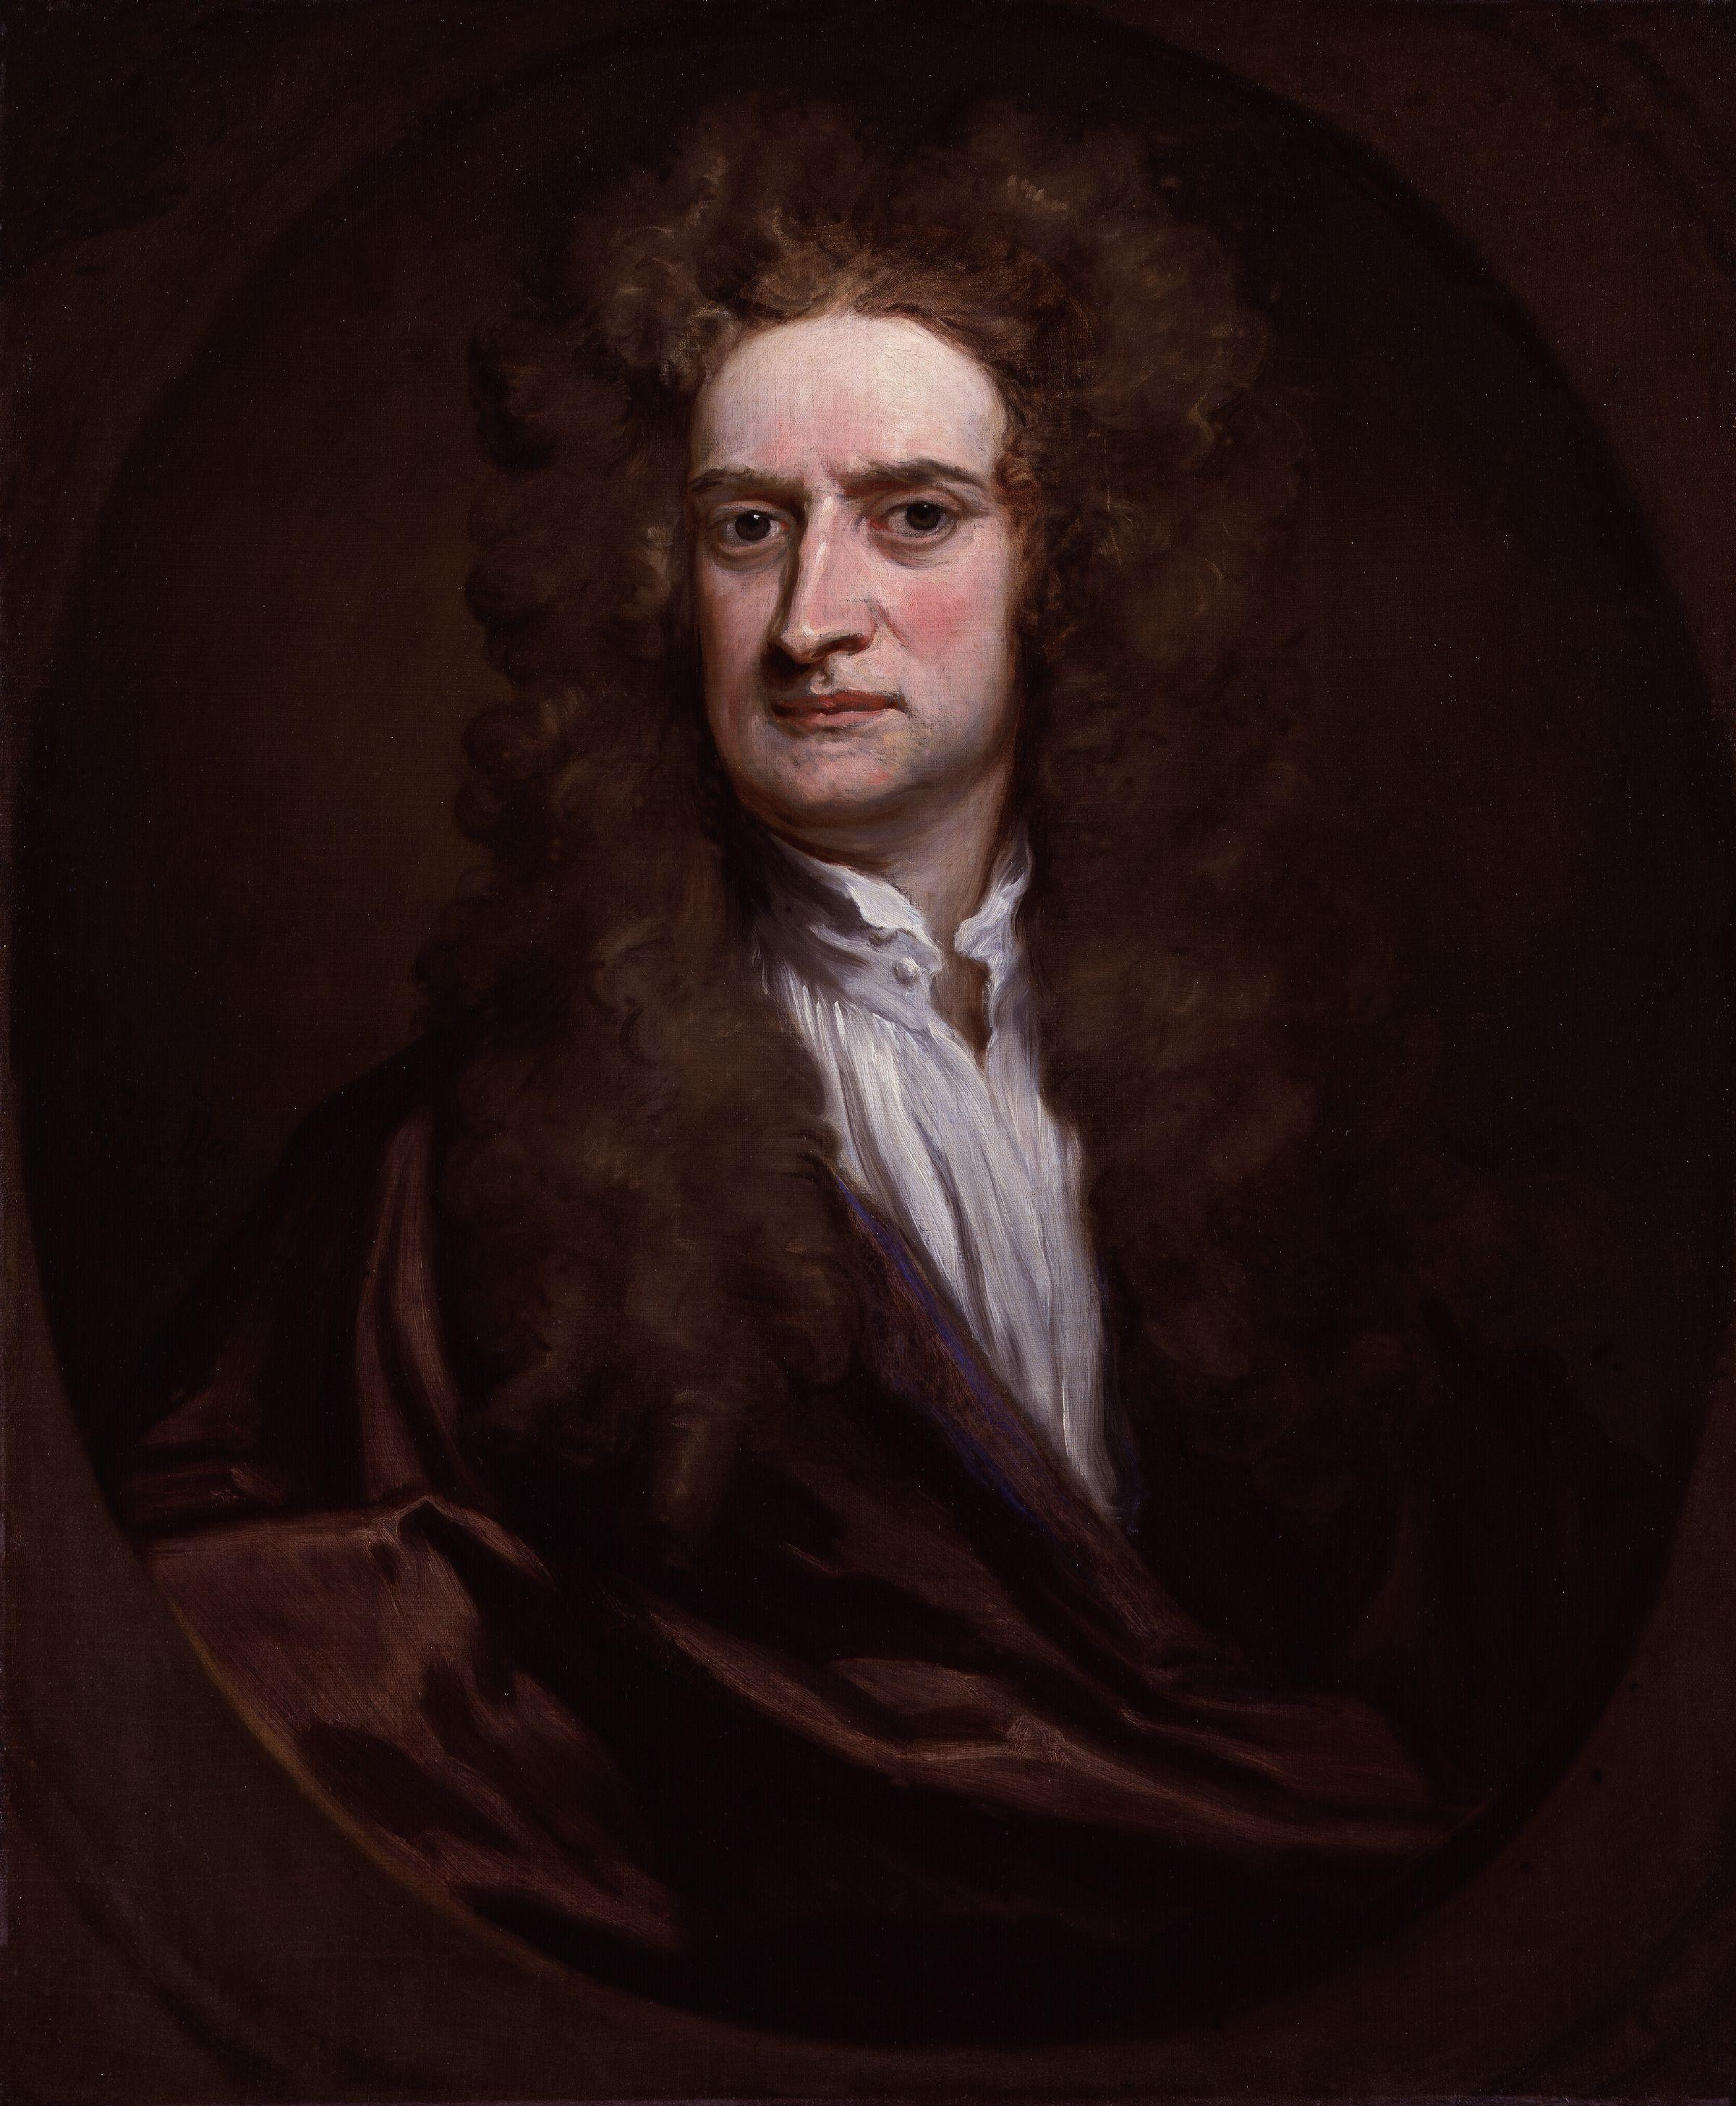
\includegraphics[height=.6\pdfpageheight]{newton.jpg}\cr
	Isaac Newton\cr
	1643--1726\cr
	}}%
	\hfil
	}
\end{frame}


\begin{frame}
\frametitle{Terminologie, etymologie, příklady}
\pause
\begin{itemize}
	\item diferenciální počet + integrální počet \pause = kalkulus \pause (\uv{počet})\pause
	\item kalkulus $\subset$ matematická analýza\pause
	\item původně jde o \emph{kalkulus nekonečně malých veličin}, \pause nyní prostě kalkulus
	\medskip
	\pause
	\item diferenciální $\sim$ \pause diference = \pause rozdíl, změna
\end{itemize}
\bigskip\pause
Kromě veličin samotných zkoumáme i jejich \alert{změny}.

\medskip\pause
Příklady?
\end{frame}


\section{Diferenciální počet}

\begin{frame}
\frametitle{Jdeme na věc}
\end{frame}

\begin{frame}
\frametitle{Leibniz podruhé}
\begin{tikzpicture}
\node (lbz) at (0,0) {\includegraphics[height=.6\pdfpageheight]{leibniz.jpg}};
\node [fill=red!30, ellipse callout, 
    callout absolute pointer={(0.50, 0.8)}]
      at (5,2) {\vbox{\hsize=.5\hsize 
			\begin{center}
			\textbf{Nova methodus pro maximis et minimis}, itemque tangentibus, quae nec fractas nec irrationales quantitates moratur, et singulare pro illis calculi genus.
			\end{center}
			}};
\end{tikzpicture}
%Nova methodus pro maximis et minimis, itemque tangentibus, quae nec fractas nec irrationales quantitates moratur, et singulare pro illis calculi genus.
\pause
\vbox{}
\vskip-2cm
\vbox{}
\begin{flushright}
Příklady?
\end{flushright}

\end{frame}

\end{document}
